\documentclass[]{scrreprt}
\usepackage{arbeitsblatt}

\title{Informatik - G11}
\ohead{Datum:...................}
\ihead{Klasse:...........}


\begin{document}
\section*{Fertiges Perzeptron testen}

\begin{center}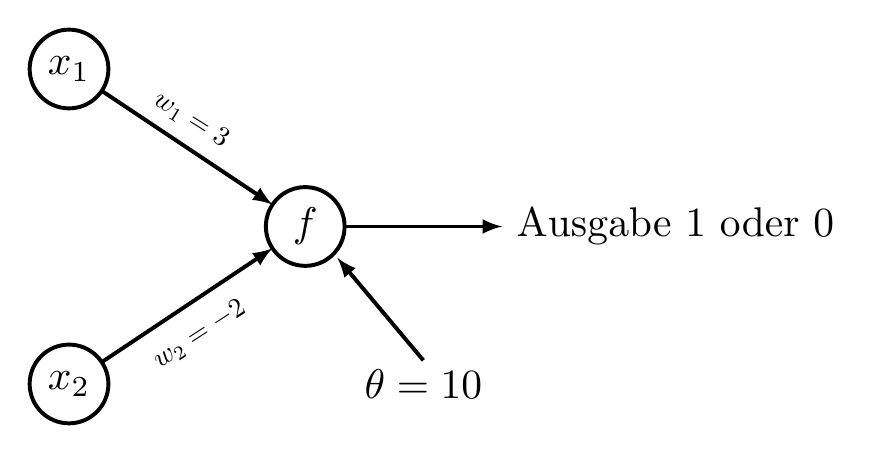
\begin{tikzpicture}


%\draw(0,0) grid ++ (12,9);



%\draw[rounded corners, fill=red!50](3,2) rectangle ++(2,6);
%\draw[rounded corners, fill=green!50](6,2) rectangle ++(2,6);


\begin{scope}[yshift=7cm]
\draw[line width=0.5mm](4,0) circle (0.5) node[scale=1.5]{$x_1$};
\end{scope}


\begin{scope}[yshift=3cm]
\draw[line width=0.5mm](4,0) circle (0.5) node[scale=1.5]{$x_2$};
\end{scope}



\begin{scope}[xshift=3cm,yshift=5cm]
\draw[line width=0.5mm](4,0) circle (0.5) node[scale=1.5]{$f$}; 
\end{scope}


%\node at (4,9) [scale=1.5]{ \parbox{2cm}{\center Eingangs-schicht}};
%\node at (7,9) [scale=1.5]{ \parbox{2cm}{\center Ausgangs-schicht}};

\draw[>=latex, ->,line width=0.5mm,  shorten >= 0.5cm, shorten <=0.50cm  ](4.,7) --  (7,5);
\draw[>=latex, ->,line width=0.5mm,  shorten >= 0.5cm, shorten <=0.50cm  ](4.,3) --  (7,5);
\draw[>=latex, ->, line width=0.5mm] (7.5, 5) -- ++(2,0);

\node at (9.5,5) [right,scale=1.5]{Ausgabe 1 oder 0}; 
\node at (5.,6.7)  [right,scale=1 , rotate=-32]{$w_1=3$};
\node at (5,3.2) [right,scale=1, rotate=33]{$w_2=-2$};


\node at (8.5,3) [scale=1.5]{$\theta=10$};
\draw[>=latex, ->, line width=0.5mm] (8.5,3.3) -- ++ (130:1.7);

\end{tikzpicture}
\end{center} 


\begin{lstlisting}
import matplotlib.pyplot as plt
from random import random

w1 = 3       # Nur Beispielwerte
w2 = -2
s = 10

x1 = float(input("x1 eingeben: "))
x2 = float(input("x2 eingeben: "))

if w1*x1+w2*x2 >= s:
  plt.scatter(x1,x2, color="green")
else:
  plt.scatter(x1,x2, color="red")

plt.show()
\end{lstlisting}

\newpage

\section*{Verbesserte Version}

Teste verschiedene Gewichte und Schwellenwerte 

\begin{lstlisting}
import matplotlib.pyplot as plt
from random import random

w1 = 3
w2 = -2
s = 0.5

def entscheidung(x1, x2):
    if w1 * x1 + w2 * x2 > s:
        return "red"
    return "green"

x = []
y = []
farben = []

for i in range(1000):
    x1 = random()  # Zahlen zwischen 0 und 1
    x2 = random()

    x.append(x1)
    y.append(x2)
    farben.append(entscheidung(x1, x2))
    
plt.scatter(x, y, color=farben)
plt.grid(True)
plt.show()
\end{lstlisting}
\end{document}
